\subsubsection*{Le matin :}
La matinée a été passée a encapsuler la regression des utilitées.

\subsubsection*{L'après midi :}
On peut désormais apprendre la fonction avec les utilitées.
Le calcul est lancé sur le cluster, en fonction des résultats la fonction de choquet sera peut être implementée.
Voici le resultat ave les utilitées:
\begin{figure}[H]
    \center
    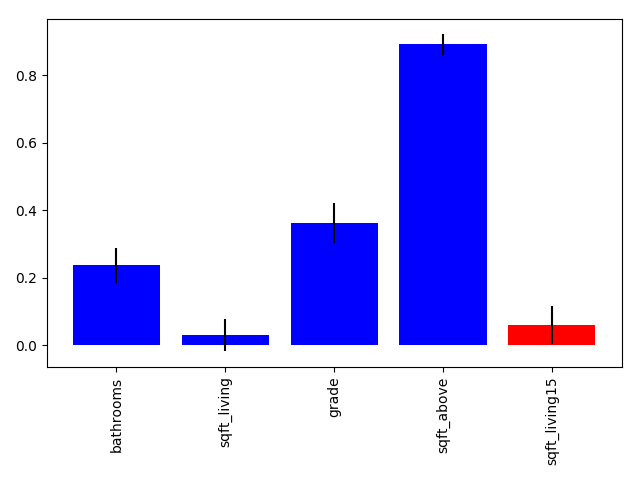
\includegraphics[height=\petit]{sources/data/Obj2/real/graphs/ut1_100_100.png}
    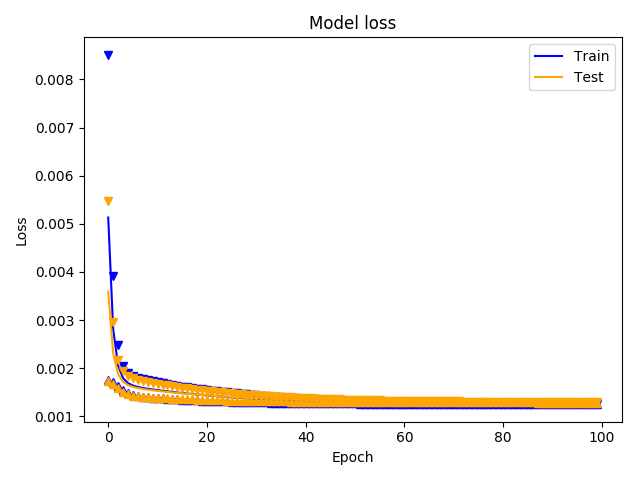
\includegraphics[height=\petit]{sources/data/Obj2/real/graphs/ut1_100_100_learn.png}
	\caption{Apprentissage sur les données réelles}
	\label{ut1_100_100}
\end{figure}
On peut voir que l'aprentissage est bien moins chaotique.
Il faudrait cependant retirer $sqft\_living$ ou $sqft\_living15$
car ils sont en compétition.
